\documentclass[aspectratio=169]{beamer}
\setbeamertemplate{navigation symbols}{}
\usepackage{color, amsmath, comment, subfigure}
\usepackage{url}

\usepackage{hyperref}
\hypersetup{
    colorlinks=true,
    linkcolor=blue,
    filecolor=magenta,      
    urlcolor=cyan,
}

%%%%%%%%%%%%%%%%%%%%%%%%%%
\title[]{Class slides for Thursday, October 8:\\Social fads, part 2}
\author[]{Matthew J. Salganik}
\institute[]{}
\date[]{COS 597E/SOC 555 Limits to prediction\\Fall 2020, Princeton University}

\begin{document}
%%%%%%%%%%%%%%%%%%%%%%%%%%%
\frame{\titlepage}
%%%%%%%%%%%%%%%%%%%%%%%%%%%
\begin{frame}

\begin{center}
  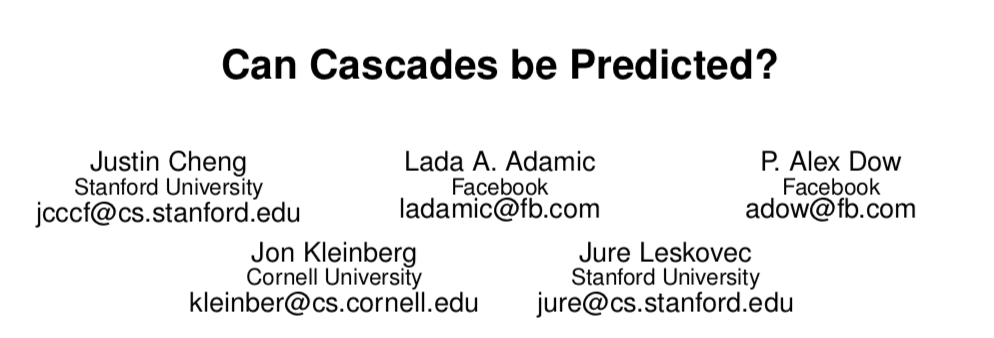
\includegraphics[width = 0.9\textwidth]{figures/cheng_can_2014_title}
\end{center}

\end{frame}
%%%%%%%%%%%%%%%%%%%%%%%%%%%%
\begin{frame}

\begin{itemize}
\item \emph{cascade growth prediction problem:} given a cascade that currently has size $k$, will it grow beyond the median size $f(k)$? \pause In this setting, this is equivalent in this setting to: given that a cascade has size $k$ will it grow beyond $2k$? 
\pause
\begin{itemize}
\item prediction problems that are balanced
\item creates one prediction problem for each $k$
\item it closely approximates real tasked needing to be solved for managing viral content
\end{itemize}
\end{itemize}

\end{frame}
%%%%%%%%%%%%%%%%%%%%%%%%%%%%
\begin{frame}

\begin{center}
  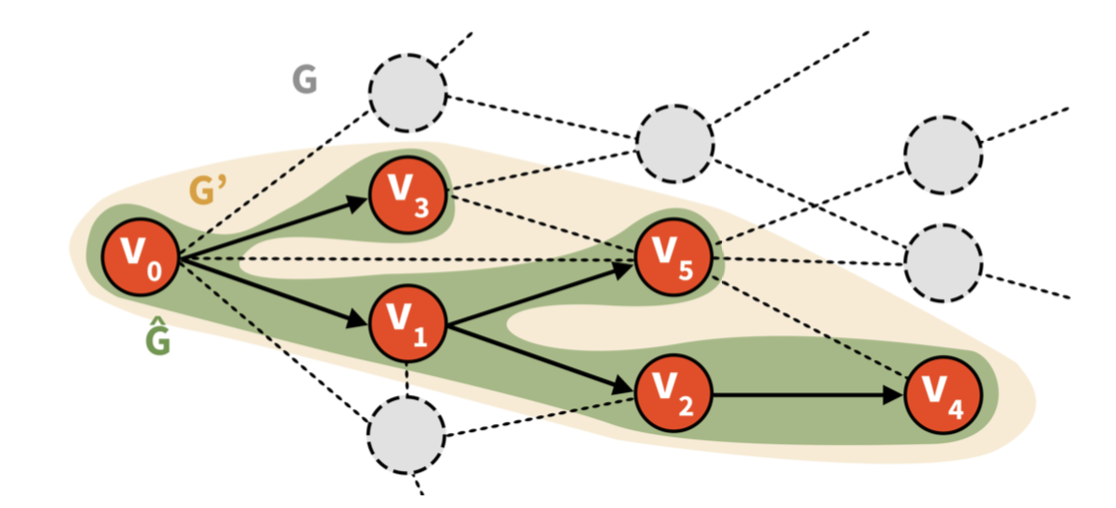
\includegraphics[width = 0.9\textwidth]{figures/cheng_can_2014_fig1}
\end{center}

\end{frame}
%%%%%%%%%%%%%%%%%%%%%%%%%%%%
\begin{frame}

\begin{columns}[c]
  \column{.5\textwidth}
  \begin{center}
    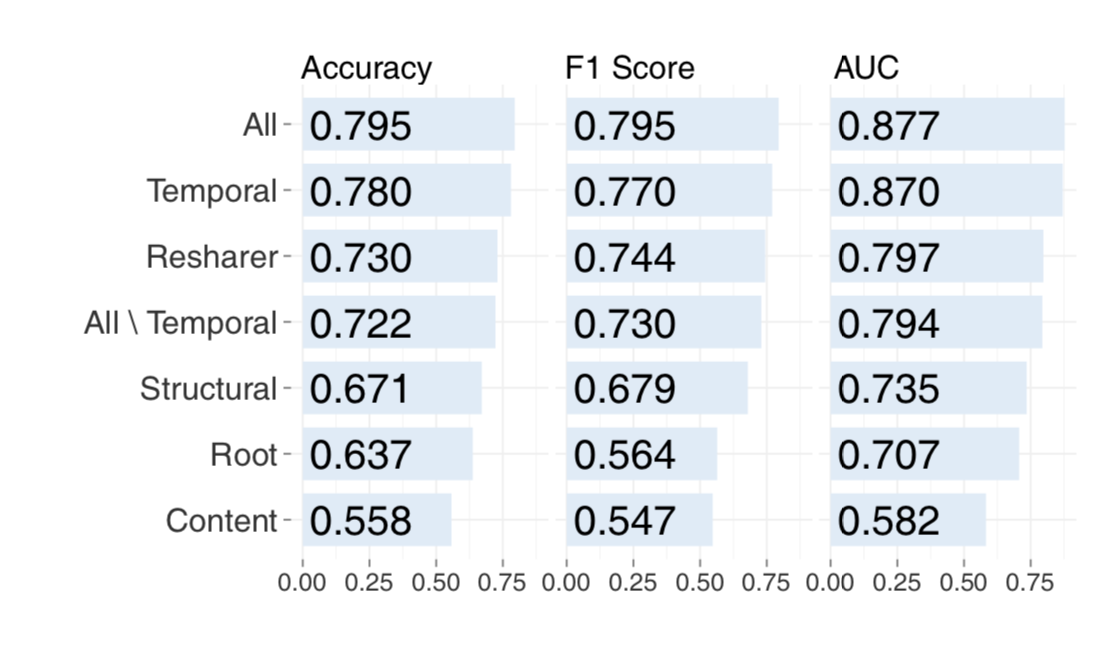
\includegraphics[width = 0.9\textwidth]{figures/cheng_can_2014_fig4}
   \end{center}
    \column{.5\textwidth} \pause
   \begin{center}
     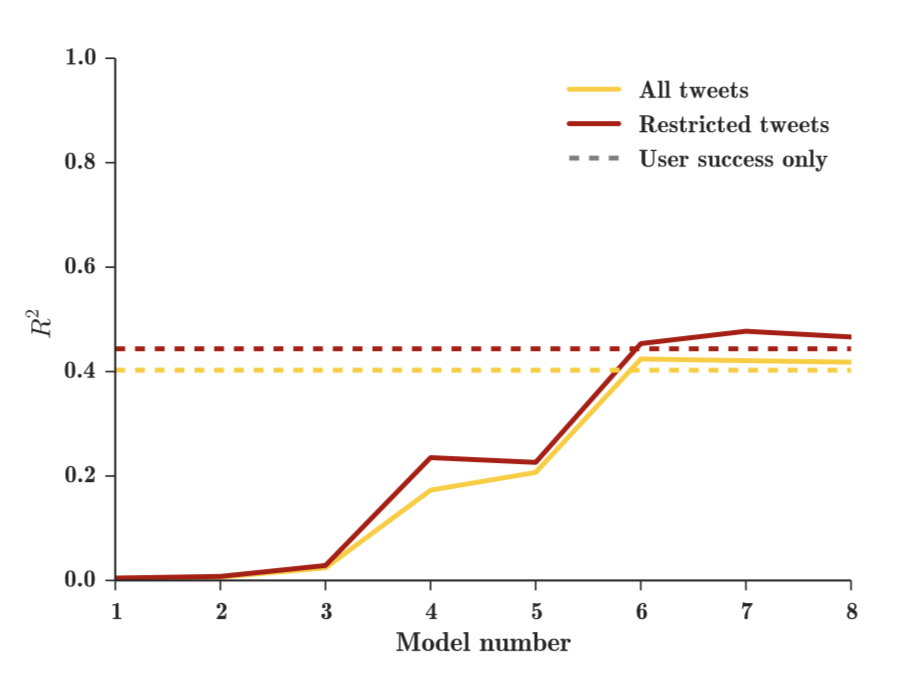
\includegraphics[width = 0.9\textwidth]{figures/martin_exploring_2016_fig4}
    \end{center}
\end{columns}

One (set) of pretty basic features does about as well as lots of features.  Does this imply that we are close to a limit?

\end{frame}
%%%%%%%%%%%%%%%%%%%%%%%%%%%%
\begin{frame}

\begin{center}
  \only<1>{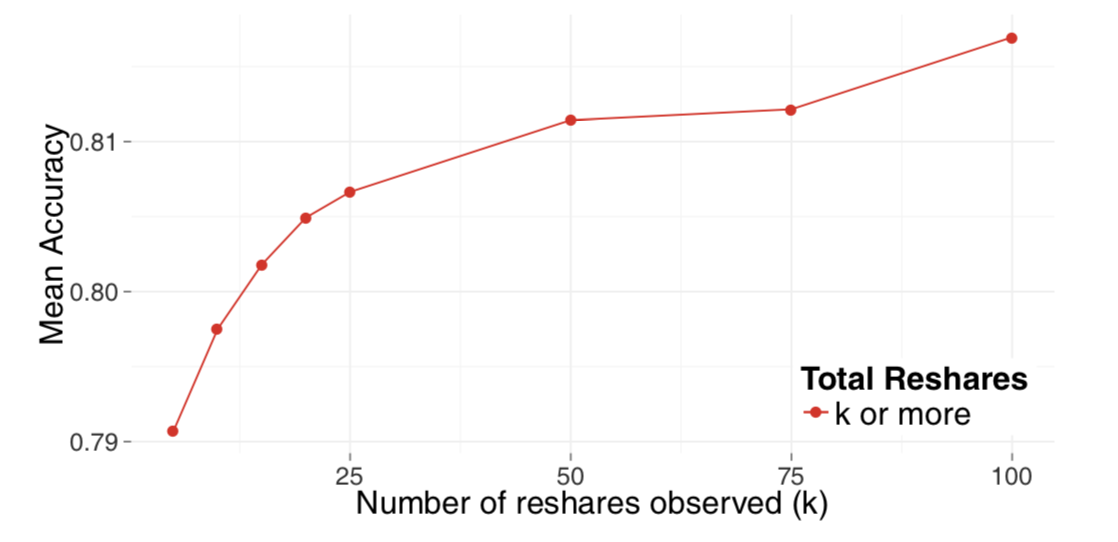
\includegraphics[width = 0.9\textwidth]{figures/cheng_can_2014_fig5}}%
  \only<2>{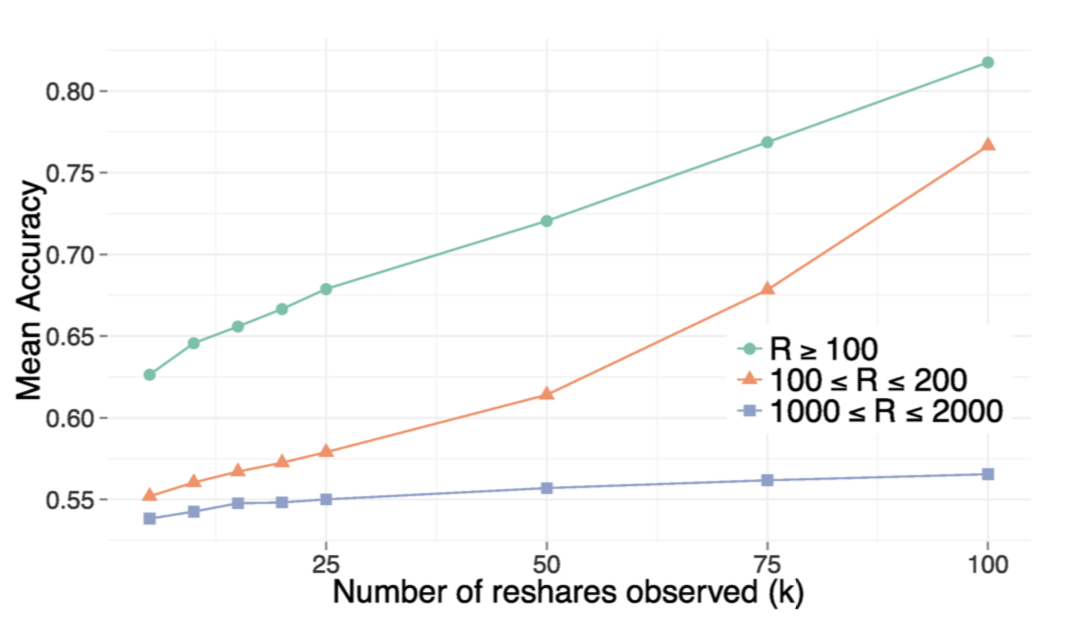
\includegraphics[width = 0.9\textwidth]{figures/cheng_can_2014_fig6}}%
\end{center}

How could we apply this same idea to other domains?  

\end{frame}
%%%%%%%%%%%%%%%%%%%%%%%%%%%%
\begin{frame}

\begin{center}
  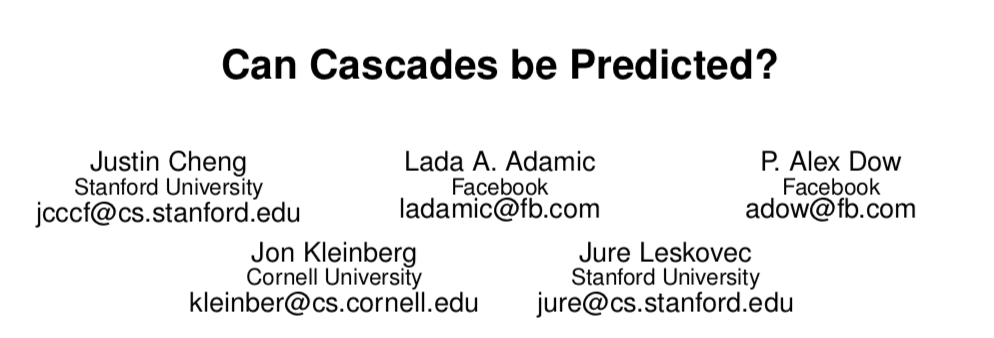
\includegraphics[width = 0.9\textwidth]{figures/cheng_can_2014_title}
\end{center}

\end{frame}
%%%%%%%%%%%%%%%%%%%%%%%%%%%%
\begin{frame}

\begin{figure}
  
\includegraphics[width = 0.9\textwidth]{figures/goel_predicting_2010_title}
\end{figure}

\end{frame}
%%%%%%%%%%%%%%%%%%%%%%%%%%%%%%%%%
\begin{frame}

\begin{center}
  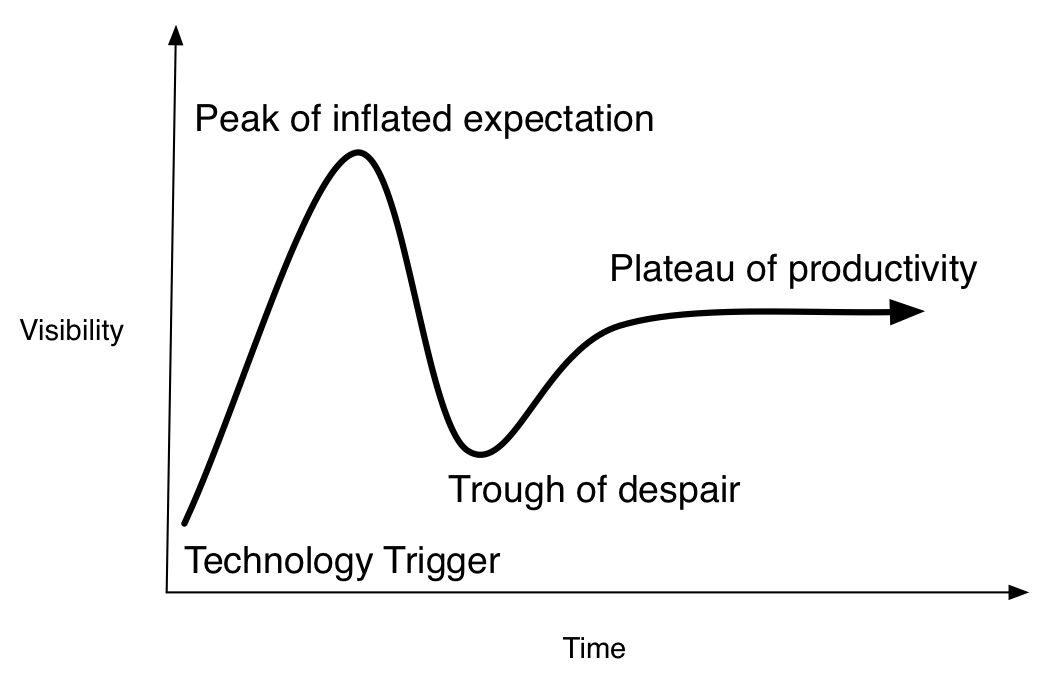
\includegraphics[width = 0.8\textwidth]{figures/hype_cycle}
\end{center}

\vfill
\url{https://en.wikipedia.org/wiki/Hype_cycle}

\end{frame}
%%%%%%%%%%%%%%%%%%%%%%%%%%%%%%%%%
\begin{frame}

\begin{center}
  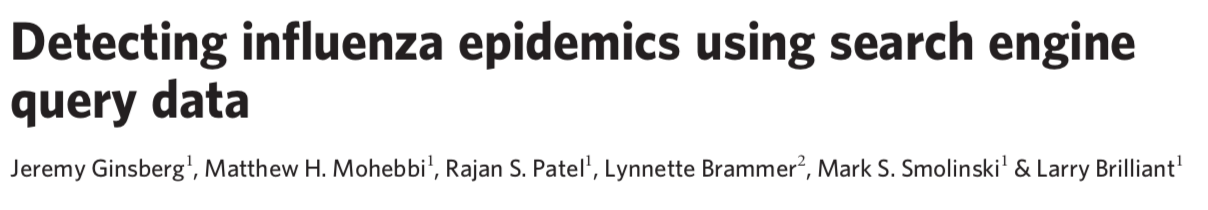
\includegraphics[width = 0.9\textwidth]{figures/ginsburg_detecting_2008_title}
\end{center}

\end{frame}
%%%%%%%%%%%%%%%%%%%%%%%%%%%%%%%%%
\begin{frame}

\begin{center}
  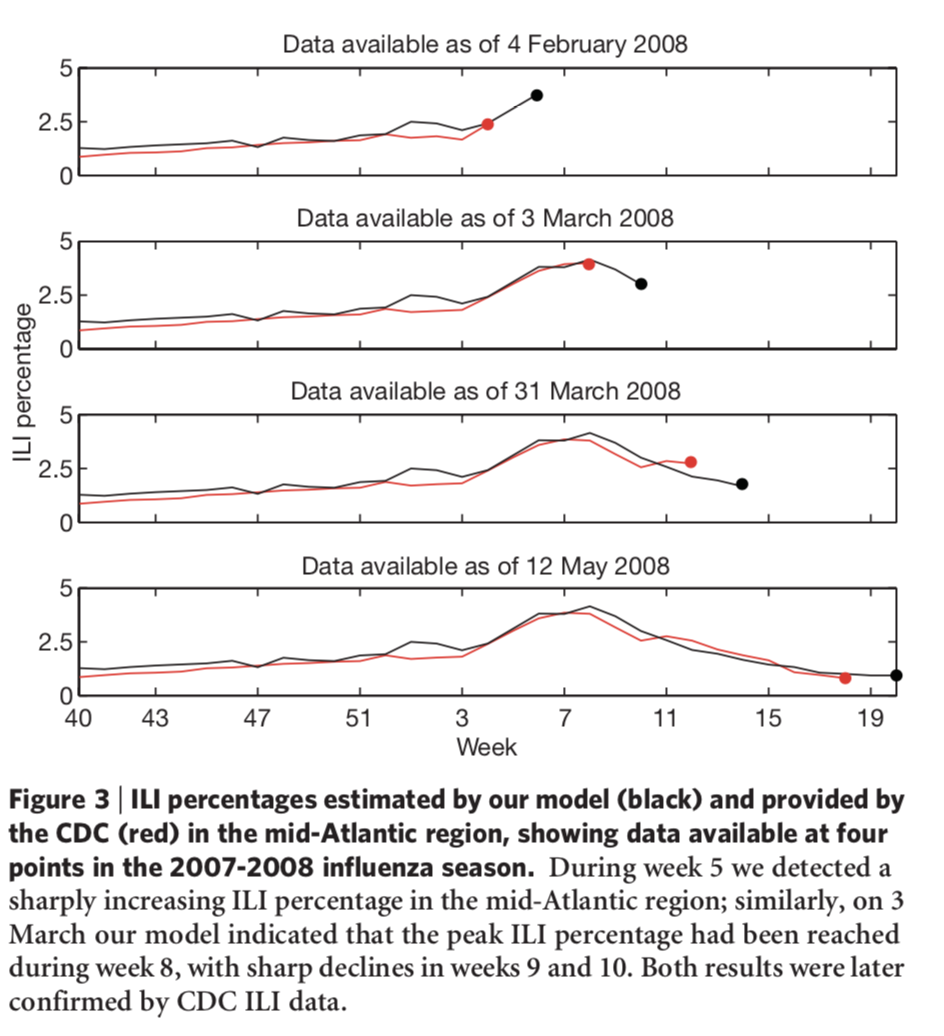
\includegraphics[height = 0.9\textheight]{figures/ginsburg_detecting_2008_fig3}
\end{center}

\end{frame}
%%%%%%%%%%%%%%%%%%%%%%%%%%%%%%%%%
\begin{frame}

\begin{center}
  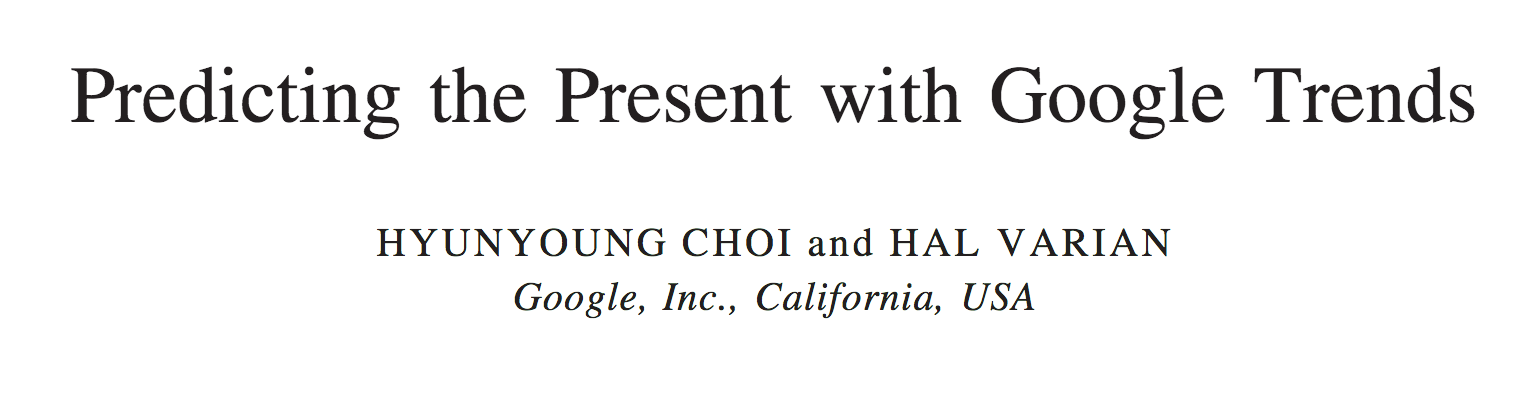
\includegraphics[width = 0.9\textwidth]{figures/choi_predicting_2012_title}
\end{center}

\end{frame}
%%%%%%%%%%%%%%%%%%%%%%%%%%%%%%%%%
\begin{frame}

\begin{center}
  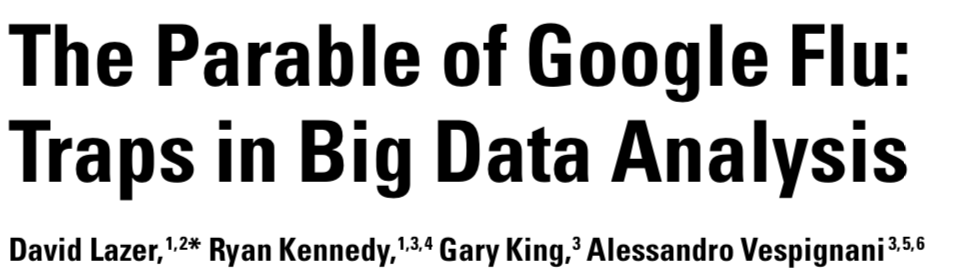
\includegraphics[width = 0.9\textwidth]{figures/lazer_parable_2014_title}
\end{center}

\end{frame}
%%%%%%%%%%%%%%%%%%%%%%%%%%%%%%%%%
\begin{frame}

\begin{center}
  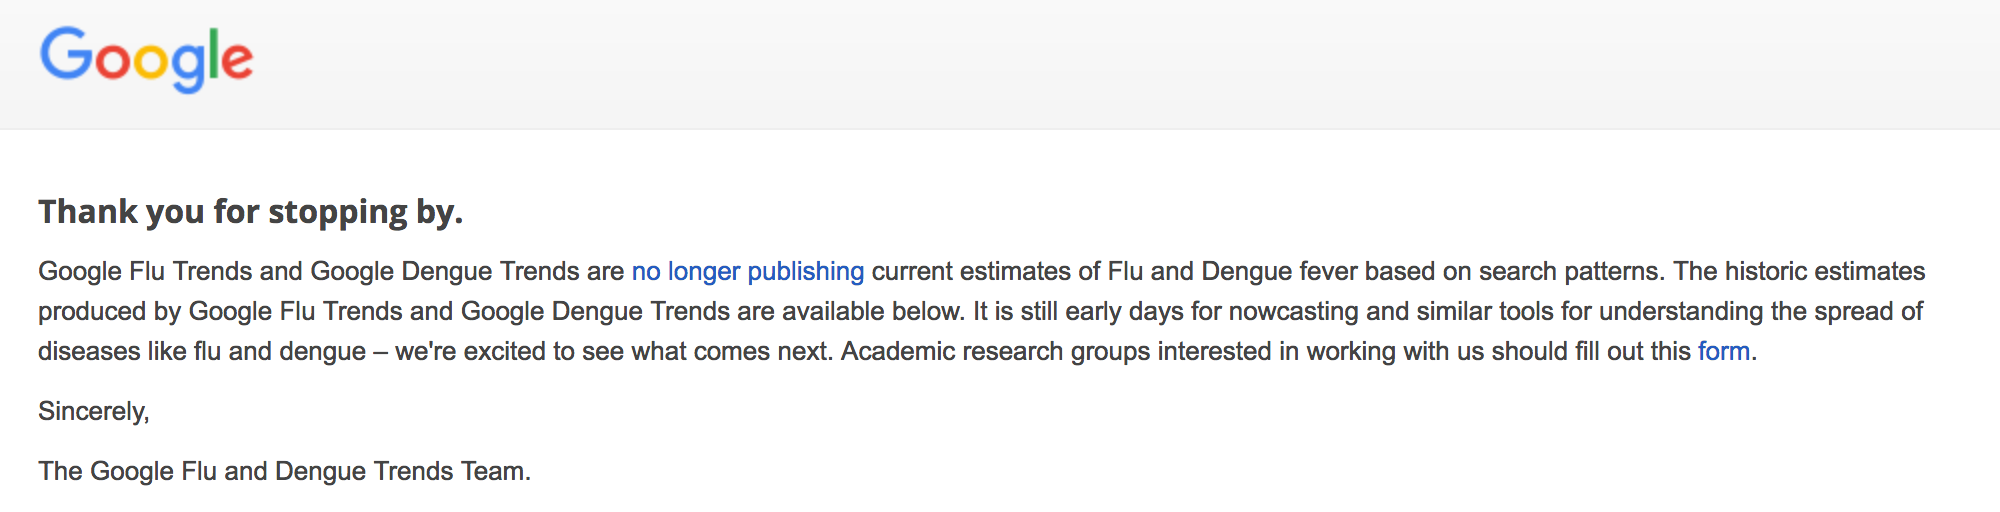
\includegraphics[width = 0.9\textwidth]{figures/google_flu_closed}
\end{center}

\vfill
Nice history: \url{https://www.theatlantic.com/technology/archive/2014/03/in-defense-of-google-flu-trends/359688/}

\end{frame}
%%%%%%%%%%%%%%%%%%%%%%%%%%%%%%%%
\begin{frame}

\begin{center}
  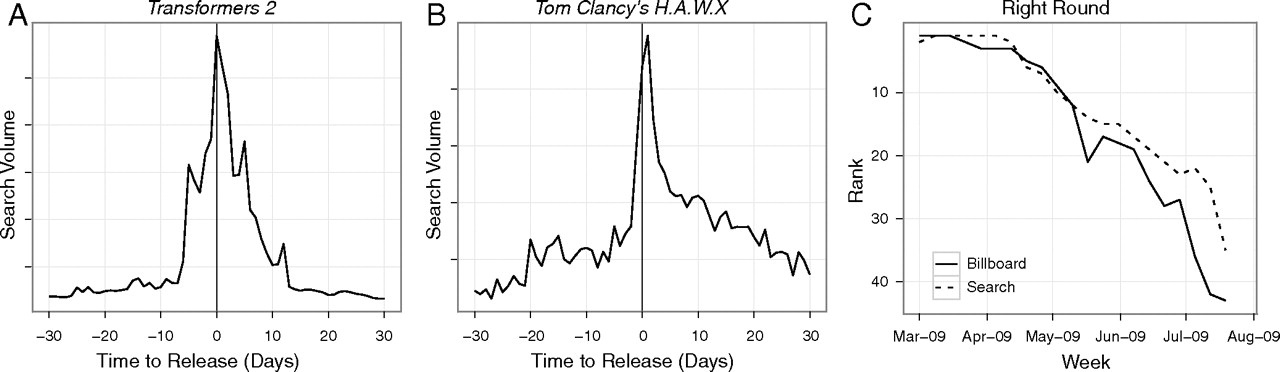
\includegraphics[width = 0.9\textwidth]{figures/goel_predicting_2010_fig1}
\end{center}

\end{frame}
%%%%%%%%%%%%%%%%%%%%%%%%%%%%%%%%%
\begin{frame}

\begin{center}
  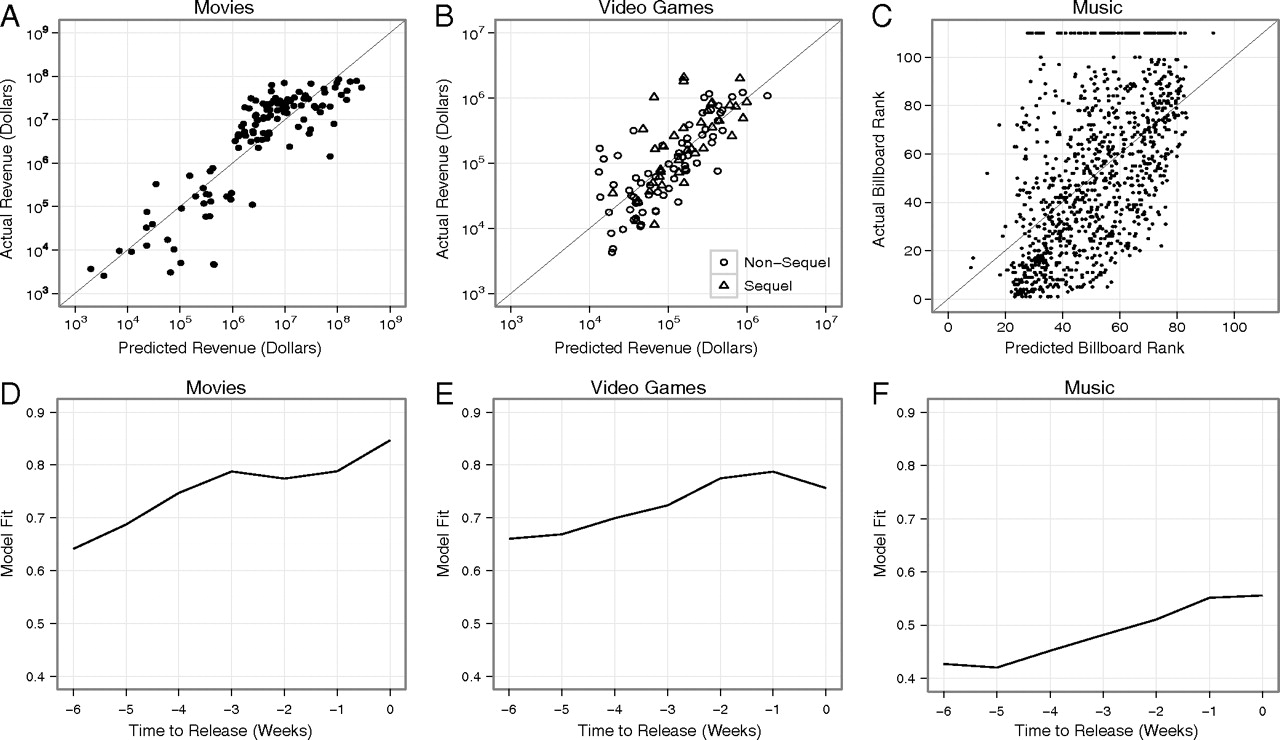
\includegraphics[width = 0.9\textwidth]{figures/goel_predicting_2010_fig2}
\end{center}

\vfill
Note that measure of predictive performance is correlation. (same as Ginsburg)
\end{frame}
%%%%%%%%%%%%%%%%%%%%%%%%%%%%%%%%%
\begin{frame}

\begin{center}
  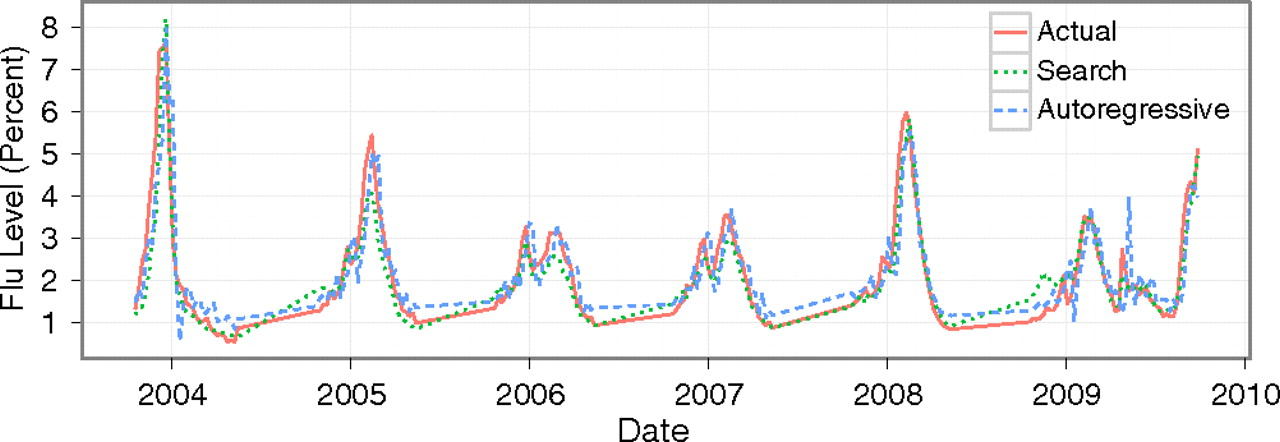
\includegraphics[width = 0.9\textwidth]{figures/goel_predicting_2010_fig4}
\end{center}

correlation between prediction and truth
\begin{itemize}
\item simple auto-regressive model: 0.86
\item Google Flu Trends: 0.94
\end{itemize}

\end{frame}
%%%%%%%%%%%%%%%%%%%%%%%%%%
\begin{frame}

\begin{center}
  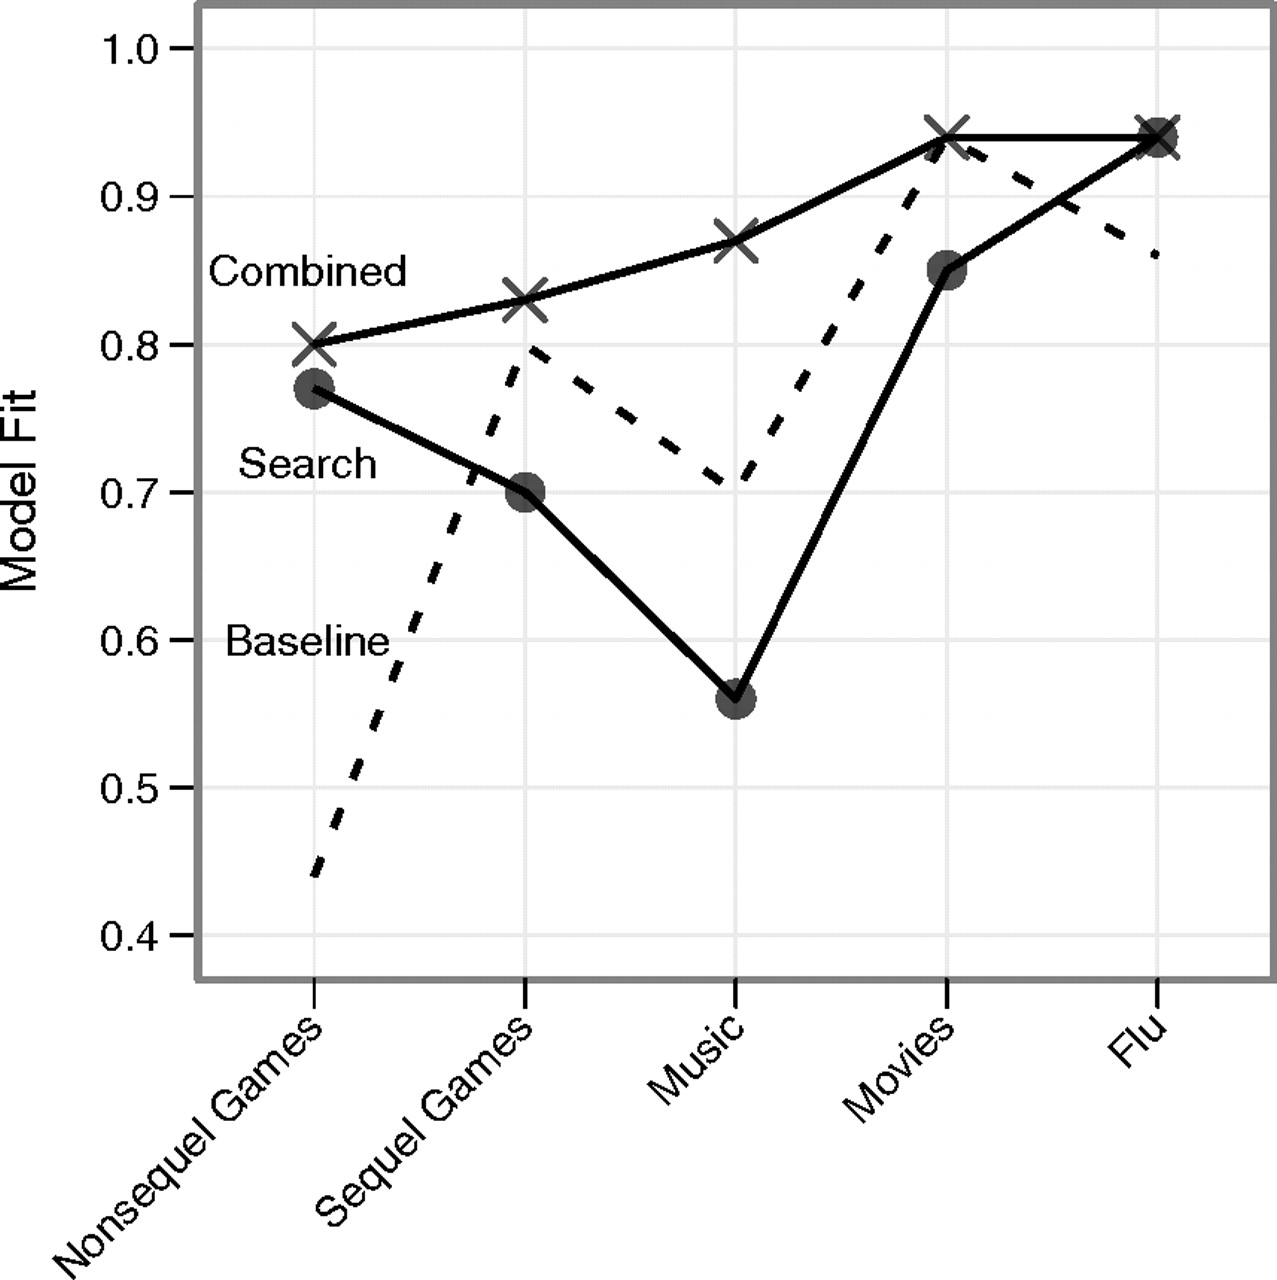
\includegraphics[width = 0.5\textwidth]{figures/goel_predicting_2010_fig5}
\end{center}

\end{frame}
%%%%%%%%%%%%%%%%%%%%%%%%%%%%
\begin{frame}

\begin{itemize}
\item For debunking: always compare to something simple
\pause 
\item Predicting the present is not the same as predicting the future
\end{itemize}

\end{frame}
%%%%%%%%%%%%%%%%%%%%%%%%%%%%%%%%%
\begin{frame}

\begin{figure}
  
\includegraphics[width = 0.9\textwidth]{figures/goel_predicting_2010_title}
\end{figure}

\end{frame}
%%%%%%%%%%%%%%%%%%%%%%%%%%%%%%%%%

\frame{\titlepage}


\end{document}
